% vim: set tw=0:
\documentclass{beamer}
\usepackage{graphicx}
\usepackage{booktabs}
\usepackage{hyperref}
\hypersetup{pdfborder={0 0 0 0}}

% Reasonable themes:
% Antibes Bergen Berkeley Berlin Frankfurt Goettingen Ilmenau Luebeck Malmoe
% Montpellier PaloAlto Rochester Singapore Szeged Warsaw bars boxes
% compatibility default lined plain shadow sidebar split tree
% And these ones include the author's name on every slide:
% Berkeley

% Declare themes.
\mode<presentation>
\usetheme{UWHEP}

% Personal macros.
\newcommand{\email}[1]{{\texttt #1}}
\newcommand{\newframe}[1]{\section{#1}
    \frametitle{\sc{#1}}}
\newcommand{\subframe}[1]{\subsection{#1}
    \frametitle{\sc{#1}}}
\newcommand{\supers}[1]{\ensuremath{^\textrm{#1}}}
\newcommand{\subs}[1]{\ensuremath{_\textrm{#1}}}
\newcommand{\ca}{\ensuremath{\sim}}
\renewcommand{\email}[1]{\href{mailto:#1}{\nolinkurl{#1}}}

% Author information.
\title{Storage at UW-Madison CMS Tier-2}
\author[Maier]{
    Will Maier \\ 
    {\tt wcmaier@hep.wisc.edu}}
\institute[Wisconsin]{University of Wisconsin - High Energy Physics}
\date[2009.06.30]{OSG Storage Forum, FNAL}
\logo{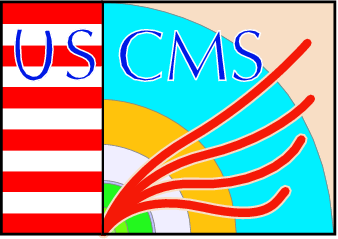
\includegraphics[height=0.6cm]{../../Graphics/USCMS_logo.png}\hspace{.1cm}
\includegraphics[height=0.75cm]{../../Graphics/UW_logo.png}}

\begin{document}

% http://indico.fnal.gov/conferenceOtherViews.py?view=standard&confId=2538
% 20 min
% Type of storage    
% Hardware
% Software configuration
% Deployment/ upgrade method
% Usage patterns
% Monitoring, troubleshooting
% Grievances
% Support expectations

\begin{frame}
    \titlepage
\end{frame}

\begin{frame}
    \tableofcontents
\end{frame}

\section{Hardware}
\subsection{Summary}
\begin{frame}
\begin{itemize}
	\item \ca{}460TB, 520 pools, 190 nodes hosting pools
	\item Most of our network architecture is provided by campus, but we manage the switches
	\item We emphasize reliability and performance on central servers
	\begin{itemize}
		\item Reliability first: performance means nothing if the systems aren't up\ldots{}
		\item \ldots{}but work doesn't get done if clients are waiting to perform lookups on the central services
	\end{itemize}
	\item Make use of any and all available machines as cluster nodes
	\begin{itemize}
		\item Dedicated servers with large, local filesystems
		\item Batch nodes
		\item Retired test systems
	\end{itemize}
\end{itemize}
\end{frame}

\subsection{Network}
\begin{frame}
\begin{itemize}
	\item 10Gbps fiber uplink to campus, world
	\item 1Gbps Ethernet to all nodes and central servers
	\item Three stacks of Cisco 3750 switches
	\begin{itemize}
		\item Main stack bridged to others via 4Gbps Etherchannel
		\item Most connections use the stack backplanes; some node-to-node and node-to-WAN connections use the Etherchannels
	\end{itemize}
	\item \ca{} 390 TB and 90 nodes on one side; 256 TB and 96 nodes on the other
	% main: g9, g10, s15, s5, opportunistic slots (45xg9x1TB, 24xg10x1.5TB, 10xs15x24TB, 9xs5x9TB)
		% 45 + 36 + 240 + 90 = 390TB
	% mr1: g7, g8 (27xg7x1TB, 5xg8x1TB)
		% 27 + 5 = 32 TB
	% mr2: g12, g14 (32xg12x3TB, 32xg14x4TB)
		% 96 + 128 = 224 TB
\end{itemize}
\end{frame}

\subsection{Central Services}
\begin{frame}
\begin{itemize}
	\item Fast RAID for namespace database
	\begin{itemize}
		\item Need speed: database journals require lots of writes
		\item Need reliability: lots of pain if the database dies or becomes corrupted
		\item At Wisconsin: LSI RAID10 (4x250 GB 10k RPM SATA disks)
	\end{itemize}
	\item Databases and dCache daemons are happy to make use of available memory and cores
	\begin{itemize}
		\item At least 2GB/core; most servers have 16GB for 4 cores
	\end{itemize}
	\item All central servers on UPS; can survive short outages or shut down gracefully
	\begin{itemize}
		\item Filesystem corruption hurts\ldots{}
	\end{itemize}
	\item Otherwise, commodity hardware
	\begin{itemize}
		\item Fewer configuration profiles to manage
		\item Standard 7200 RPM SATA disks sufficient; no RAID (only namespace needs to persist)
	\end{itemize}
\end{itemize}
\end{frame}

\subsection{Cluster nodes}
\begin{frame}
\begin{itemize}
	% XXX: table?
	\item Majority of storage on whitebox, dual-purpose batch and storage nodes
	%\item Historically, dedicated nodes have lower availability
	%\begin{itemize}
	%	\item Consequence of hardware failure is greater
	%	\item Cursed with wonky RAID controllers -- extra point of failure?
	%\end{itemize}
	\item Nodes stay in the cluster until it's too expensive to keep them running
	\begin{itemize}
		\item With five year warranties on disks, nodes can last a long time
		\item RAM upgrades or motherboard failures aren't worth the trouble if the node is out of warranty (standard three years)
	\end{itemize}
	\end{itemize}

	\begin{table}
	\begin{tabular}{rllll}
		\toprule
		Generation	& Disk (TB)	& RAM (GB)	& CPU	& Count	\\
		\midrule
		1		& XXX		& XXX		& XXX	& XXX	\\ % g7,g8
		2		& XXX		& XXX		& XXX	& XXX	\\ % g9,g10
		3		& XXX		& XXX		& XXX	& XXX	\\ % g12
		4		& XXX		& XXX		& XXX	& XXX	\\ % g14
		5		& XXX		& XXX		& XXX	& XXX	\\ % g7,g8
		\midrule
		dedicated	& XXX		& XXX		& XXX	& XXX	\\ % s5,s15
		\bottomrule
	\end{tabular}
	\caption{Wisconsin Storage Cluster Nodes, 2005-2009}
	\label{cluster_nodes}
	\end{table}

	% XXX: pie chart dedicated vs not (google charts?)
\begin{itemize}
	\item Dedicated storage
	\begin{itemize}
		\item Apple Xserve RAID, 9TB, fiber channel
		\item Whitebox 24 TB local SATA disks, LSI RAID6
	\end{itemize}
\end{itemize}
\end{frame}

\section{Software}
\subsection{Central Services}
\begin{frame}
\begin{itemize}
	\item Originally six central servers, with one service on each machine
	\item Now, dedicated nodes for PNFS, 'admin' services, SRM/dcap
	\item Hotspare system running and ready to cover for any of the above
	\item Databases running on all servers
	\begin{itemize}
		\item Logging disabled
	\end{itemize}
	\item PNFS
	\begin{itemize}
		\item companion database
		\item XXX PFM replication (for fast namespace lookups)
	\end{itemize}
	\item admin
	\begin{itemize}
		\item XXX http monitor, admin interface, companion and billing databases
		\item Admin interface configured with SSH keys
		\item {\tt billingrep} live replicator (for access to the billing log)
	\end{itemize}
	\item SRM/dcap
	\begin{itemize}
		\item Only one door for each, and they live on the same machine
		\item Haven't observed performance problems
	\end{itemize}
	\item Hotspare
	\begin{itemize}
		\item {\tt /opt/d-cache} already present
		\item Ready for quick redeployment of a failed central service
	\end{itemize}
\end{itemize}
\end{frame}

\subsection{Cluster Nodes}
\begin{frame}
\begin{itemize}
	\item 30 GridFTP doors scattered across nodes
	\item Configure dCache JVMs so that 1GB RAM/core remains
	\begin{itemize}
		\item In most cases, four pool daemons, each with 400M JVMs
	\end{itemize}
	\item Most storage nodes also run Condor
	\begin{itemize}
		\item Jobs are almost always running
		\item Jobs fetching data, dCache pushing files
		% \item (1000 slots x 2MB/s)/250 storage nodes
		\item No bottlenecks (yet) on the nodes, but the Etherchannels are troublesome
	\end{itemize}
\end{itemize}
\end{frame}

\section{Administration}
\subsection{Deployment}
\begin{frame}
\begin{itemize}
	\item Configuration and installation automated by CFEngine
	\item {\tt /opt/d-cache} versioned by Mercurial, synced from AFS by CFEngine
	\item CFEngine also installs extra RPMs, mounts PNFS, etc
	\item CFEngine handles upgrades, too:
	\begin{itemize}
		\item (We don't use the VDT dCache)
		\item Merge new {\tt /opt/d-cache} with local using {\tt hg} (clean upstream branch, local branch)
		\item Turn off services
		\item Push updates to all nodes and run {\tt install.sh} (CFEngine)
		\item Start services; revert to old {\tt /opt/d-cache} if necessary
	\end{itemize}
\end{itemize}
\end{frame}

\subsection{Monitoring}
\begin{frame}
\begin{itemize}
	\item Nagios
	\item dCache Health Check
	\item SAM, RSV
	\item Stuck transfers
	\item Per-directory replication rate (walk namespace)
	\item root-owned files/directories
	\item Absent pool report
\end{itemize}
\end{frame}

\subsection{Replication}
\begin{frame}
\begin{itemize}
	\item Since we store data on commodity hardware (with no RAID), we make copies at the cluster level
	\item dCache's Replica Manager couldn't keep up with the flood of pool messages
	\begin{itemize}
		\item XXX Stopped running in 2007
	\end{itemize}
	\item PFM performance slows with lots of pools and files
	\item {\tt billingrep} for low-latency, first order replication
	\begin{itemize}
		\item Watches billing log for file creations
		\item XXX {\tt pp get file} to a random pool
		\item Files replicated within seconds
		\item Not aware of pool cost or availability; doesn't recover if replicas disappear
		\item \url{http://code.hep.wisc.edu/dcache-tools}
	\end{itemize}
	\item {\tt pfm} for accurate policy enforcement
	\begin{itemize}
		\item Walks PNFS namespace (\ca{}30 minutes for 300k files)
		\item Finds available replicas for each file and adds or removes replicas depending on policy
		\item Policy defined by regular expressions matching logical file names
		\item At Wisconsin: No more or less than two replicas for each file
	\end{itemize}
\end{itemize}
\end{frame}

\section{Experiences}
\subsection{Usage}
\begin{frame}
\begin{itemize}
	\item Very few files lost (thanks to replication)
	\item Adequate performance in LoadTest
	\item Without fast disks on PNFS node, transfer pileups
	\item XXX users, XXX simultaneous transfers
	\item Merging lots of small files hurts
	\item Highly efficient analysis of large files (relatively small overhead)
\end{itemize}
\end{frame}

\subsection{Workflows}
\begin{frame}
\begin{itemize}
	\item Most local workflows involve extended analysis of large files or merging many small files
	\item Analysis:
	\begin{itemize}
		\item dCache works well without much modification
		\item Small overhead per transfer, dcap provides fast access
		\item Relatively few outputs for each job
	\end{itemize}
	\item Merge:
	\begin{itemize}
		\item More common with SLHC
		\item Most approaches merge numerous small files in serial
		\item Unavailable files wait for timeout; during peak usage, time to fetch available files exceeds reasonable timeouts
		\item Improving PNFS performance helps, but this workflow is still inefficient on dCache
	\end{itemize}
\end{itemize}
\end{frame}

\subsection{Plans}
\begin{frame}
\begin{itemize}
	\item Centralize databases on high-performance server or provide faster disks on all central servers
	\item Improve switch port efficiency so all nodes communicate across the same 16Gbps backplane
	\item Expand UPS coverage
	\item {\tt pgpool} replication of PostgreSQL databases
	\item Point {\tt billingrep} at database, not log
	\item Local test stand/verify upgrades
	\item Multiple dcap doors
\end{itemize}
\end{frame}

\end{document}
